% Flow network
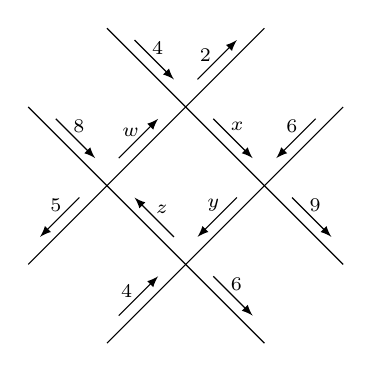
\begin{tikzpicture}

	\draw (0,1) to (3,4);
	\draw[-latex] (0.65,1.85) to node[anchor=south, pos=0.6] {$\scriptstyle 5$} (0.15,1.35);
	\draw[-latex] (1.15,2.35) to node[anchor=south, pos=0.3] {$\scriptstyle w$} (1.65,2.85);
	\draw[-latex] (2.15,3.35) to node[anchor=south, pos=0.2] {$\scriptstyle 2$} (2.65,3.85);

	\draw (1,0) to (4,3);
	\draw[-latex] (1.15,0.35) to node[anchor=south, pos=0.2] {$\scriptstyle 4$} (1.65,0.85);
	\draw[-latex] (2.65,1.85) to node[anchor=south, pos=0.6] {$\scriptstyle y$} (2.15,1.35);
	\draw[-latex] (3.65,2.85) to node[anchor=south, pos=0.6] {$\scriptstyle 6$} (3.15,2.35);

	\draw (0,3) to (3,0);
	\draw[-latex] (0.35,2.85) to node[anchor=west,pos=0.2] {$\scriptstyle 8$} (0.85,2.35);
	\draw[-latex] (1.85,1.35) to node[anchor=west,pos=0.7] {$\scriptstyle z$} (1.35,1.85);
	\draw[-latex] (2.35,0.85) to node[anchor=west,pos=0.2] {$\scriptstyle 6$} (2.85,0.35);

	\draw (1,4) to (4,1);
	\draw[-latex] (1.35,3.85) to node[anchor=west,pos=0.2] {$\scriptstyle 4$} (1.85,3.35);
	\draw[-latex] (2.35,2.85) to node[anchor=west,pos=0.2] {$\scriptstyle x$} (2.85,2.35);
	\draw[-latex] (3.35,1.85) to node[anchor=west,pos=0.2] {$\scriptstyle 9$} (3.85,1.35);

\end{tikzpicture}
